%-------------------------------%
% Template modify from Alexander Soen's Student Assignment Template
%https://www.overleaf.com/latex/templates/student-assignment-template/sjkprrdkmphg
%-------------------------------%

\documentclass[a4paper]{article}
\usepackage{student}
\usepackage{float}

% Metadata
\date{\today}
\setmodule{Assignment 3 Report}
\setterm{115-1 (Fall 2026)}

%-------------------------------%
% Other details
% TODO: Fill the information
%-------------------------------%
\title{Reinforcement Learning}
\setmembername{YOUR-NAME} % In English
\setmemberuid{YOUR-UID}
%-------------------------------%
% Add / Delete commands and packages
% TODO: Add / Delete here as you need
%-------------------------------%
\usepackage{amsmath,amssymb,bm}

\newcommand{\KL}{\mathrm{KL}}
\newcommand{\R}{\mathbb{R}}
\newcommand{\E}{\mathbb{E}}
\newcommand{\T}{\top}

\newcommand{\expdist}[2]{%
        \normalfont{\textsc{Exp}}(#1, #2)%
    }
\newcommand{\expparam}{\bm \lambda}
\newcommand{\Expparam}{\bm \Lambda}
\newcommand{\natparam}{\bm \eta}
\newcommand{\Natparam}{\bm H}
\newcommand{\sufstat}{\bm u}

% Main document
\begin{document}
    % Add header
    \header{}
    \section{2048}
    % Use `answer` environment to add solutions
    % \begin{answer}[Question 1.1] for example starts an environment formatted
    % for Question 1.1
    \begin{answer}[Q1. Given $\pi = argmaxQ$, implement Monte Carlo evaluation of $Q^\pi(s,a)$. State how you handle tile-spawn randomness, the number of rollouts, and confidence intervals. (3 pts.) ]
        Your answer here.

        An equation with numbering:
        \begin{equation}
            \expdist{\sufstat}{\natparam}.
        \end{equation}

        An equation without numbering (notice the $*$):
        \begin{equation*}
            \expparam^{\T} \sufstat(x).
        \end{equation*}
    \end{answer}

    \begin{answer}[Q2. For DQN and DDQN, plot predicted Q against MC-estimated $Q^\pi$ on states visited by $\pi$. Is there a discrepancy? Explain the difference between the two algorithms. Does a small discrepancy imply a good policy? (5 pts.)]
        Your answer here.

        \begin{figure}[H]
            \centering
            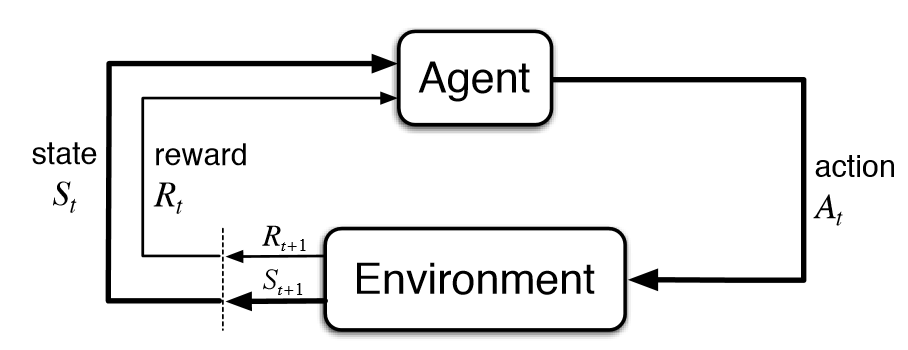
\includegraphics[width=0.5\textwidth]{images/RL_framework.png}
            \caption{Caption}
            \label{fig:enter-label}
        \end{figure}
        
        An equation with numbering:
        \begin{equation}
            \expdist{\sufstat}{\natparam}.
        \end{equation}

        An equation without numbering (notice the $*$):
        \begin{equation*}
            \expparam^{\T} \sufstat(x).
        \end{equation*}
    \end{answer}
    \begin{answer}[Q3. Describe how you trained your best model (architecture, reward, tricks). (4 pts.)]
        Your answer here.

        An equation with numbering:
        \begin{equation}
            \expdist{\sufstat}{\natparam}.
        \end{equation}

        An equation without numbering (notice the $*$):
        \begin{equation*}
            \expparam^{\T} \sufstat(x).
        \end{equation*}
    \end{answer}
    \section{Astro Party}
    \begin{answer}[Q4. Thoroughly describe your pipeline for best performance (Be creative! Any technique is worth sharing!) (9 pts.)]
        Your answer here.

        An equation with numbering:
        \begin{equation}
            \expdist{\sufstat}{\natparam}.
        \end{equation}

        An equation without numbering (notice the $*$):
        \begin{equation*}
            \expparam^{\T} \sufstat(x).
        \end{equation*}
    \end{answer}
    \begin{answer}[Q5. Try at least 2 RL algorithms from SB3, explain why one works better than the other. State at least one hypothesis and do clean experiments to justify/falsify them. (9 pts.)]
        Your answer here.

        \begin{figure}[H]
            \centering
            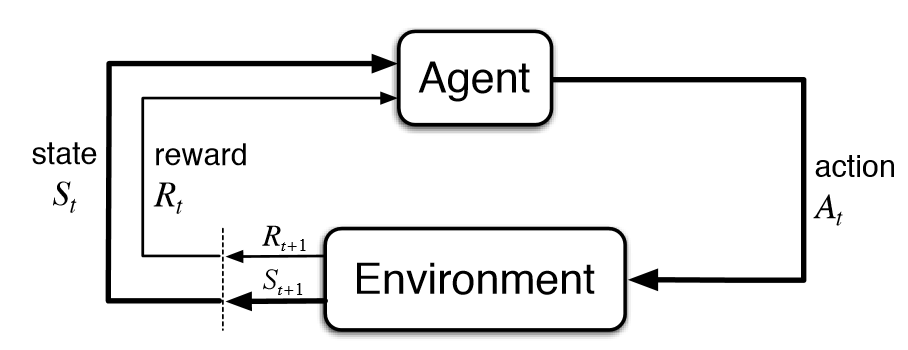
\includegraphics[width=0.5\textwidth]{images/RL_framework.png}
            \caption{Caption}
            \label{fig:enter-label}
        \end{figure}
        
        An equation with numbering:
        \begin{equation}
            \expdist{\sufstat}{\natparam}.
        \end{equation}

        An equation without numbering (notice the $*$):
        \begin{equation*}
            \expparam^{\T} \sufstat(x).
        \end{equation*}
    \end{answer}
\end{document}
